\section[Sampling And Visualization]{抽样与可视化}\label{sec:4}

\subsection[Sampling]{抽样}\label{subsec:4-1}
\begin{frame}{抽样}

\ff{
	通过前文所述的方法,根据掘进机已经驶过的区域的椭球的数据,可预测掘进机近前方区域椭球九个参数可能的分布和近前方断层的密度$\hat{d}(T+1)$。进而,对于一个尺寸为$a \times b \times c$(${\rm m}^3$)的矩形统计窗,我们可以基于预测出的这些分布的性质,抽取出$a \times b \times c \times \hat{d}(T+1)$个样本,并将其组成$a \times b \times c \times \hat{d}(T+1)$个椭球,来作为TBM近前方岩体的裂隙的分布。\\
	
	对于均匀分布、对数正态分布、指数分布的抽取,我们利用Python的\textit{random}库,该库内置了这些常见分布的随机数生成器。对于Fisher分布的抽取我们就利用近似公式\footcite{priest2012discontinuity}:
\begin{equation}\label{equ:FisherSample}
\theta - \theta_i = \Delta(\theta) = \cos^{-1}[\frac{\ln(1 - {\rm Random}(0, 1))}{\kappa}+1]
\end{equation}


}

\end{frame}

\subsection[Visualization]{可视化}\label{subsec:4-2}
\begin{frame}{可视化}

\ff{
	\alert{使用工具}对于数据的可视化我们采用免费的开源软件VTK(Visualization Toolkit,即可视化工具包)。VTK封装了很多可视化过程中常用的数据结构和算法,其中就包括椭球绘制的算法\textit{vtkParametricEllipsoid}
	
	
	\alert{绘制流程\footcite{schroeder2000visualizing, avila2010vtk}:}\\
	\begin{columns}
	\column{.5\textwidth}
	$\quad$
	\structure{步骤一:}设置椭球参数\\
	\tikzstyle{process} = [rectangle,rounded corners, minimum width=2cm,minimum height=0.5cm,text centered, draw=black,fill=gray!30]
	\tikzstyle{arrow} = [thick,->,>=stealth]

	$\quad$
	\begin{tikzpicture}[node distance=2cm]
	\node (process1) [process] {vtkParametricEllipsoid};
	\node (process2) [process, below of=process1, yshift=1cm] {vtkPolyDataMapper};
	\node (process3) [process, below of=process2, yshift=1cm] {vtkActor};
	%\node (process4) [process, below of=process3, yshift=2cm] {vtkRenderer};
	%\node (process5) [process, left of=process4, xshift=4cm] {vtkRenderWindow};

	\draw [arrow] (process1) -- (process2);
	\draw [arrow] (process2) -- (process3);
	%\draw [arrow] (process3) -- (process4);
	%\draw [arrow] (process4) -- (process5);
	\end{tikzpicture}
	
	
	\column{.5\textwidth}
	$\quad$
	\structure{步骤二:}渲染椭球\\
	\tikzstyle{process} = [rectangle,rounded corners, minimum width=2cm,minimum height=0.5cm,text centered, draw=black,fill=gray!30]
	\tikzstyle{arrow} = [thick,->,>=stealth]
	$\quad$
	\begin{tikzpicture}[node distance=2cm]
	\node (process3) [process] {vtkActor};
	\node (process4) [process, below of=process3, yshift=1cm] {vtkRenderer};
	\node (process5) [process, below of=process4, yshift=1cm] {vtkRenderWindow};

	\draw [arrow] (process3) -- (process4);
	\draw [arrow] (process4) -- (process5);
	\end{tikzpicture}\\
	
	\end{columns}
}
	
\end{frame}

\begin{frame}{样例}
	\ff{
		
	\begin{table}[!htbp]
	\caption{椭球参数分布和密度}
	\label{tab:EiilpDisDensity}
	\centering
	\footnotesize% fontsize
	\setlength{\tabcolsep}{4pt}% column separation
	\renewcommand{\arraystretch}{1.2}%row space 
	\begin{tabular}{lcccccccc}
		\hline
		椭球参数 & \multicolumn{4}{c}{不同采样段椭球参数的分布}\\
		\cline{2-5}% partial hline from column i to column j
		\hline
		& 一 & 二 & 三 & 四 \\
		$S_x$ & Exp$(0.1)$ & Exp$(0.1)$ & Exp$(0.1)$ & Log-N$(2, 4)$\\
		$S_y$ & Exp$(0.1)$ & Exp$(0.1)$ & Exp$(0.1)$ & Log-N$(2, 4)$\\
		$S_z$ & Exp$(1)$ & Exp$(1)$ & Exp$(1)$ & Log-N$(0.6, 2)$\\
		$\gamma$ & Fisher$(10)$ & Fisher$(10)$ & Fisher$(10)$ & Fisher$(10)$\\
		$\theta$ & Fisher$(10)$ & Fisher$(10)$ & Fisher$(100)$ & Fisher$(10)$\\
		样本数 & $20$ & $40$ & $20$ & $20$\\	 
		\hline
	\end{tabular}
\end{table}

}
\end{frame}

\begin{frame}{样例}
	\ff{
		\begin{figure}
		\centering
		\begin{subfigure}{样例一}
			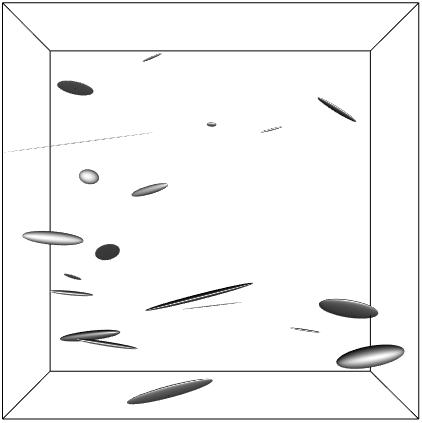
\includegraphics[width=2.5cm]{figure/visual1}
			\label{fig:visual1}
		\end{subfigure}
		~
		\begin{subfigure}{样例二}
			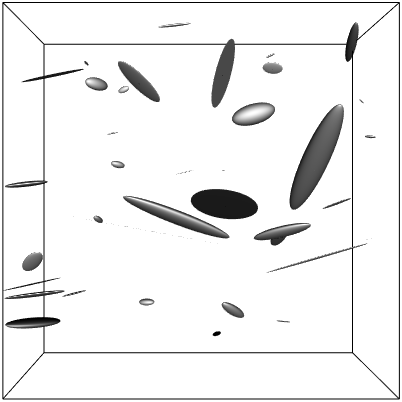
\includegraphics[width=2.5cm]{figure/visual2}
			\label{fig:visual2}
		\end{subfigure}
		\\
		\begin{subfigure}{样例三}
			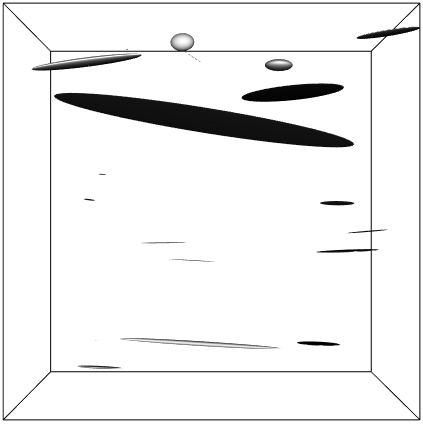
\includegraphics[width=2.5cm]{figure/visual3}
			\label{fig:visual3}
		\end{subfigure}
		~
		\begin{subfigure}{样例四}
			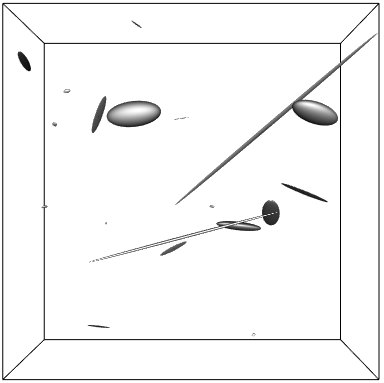
\includegraphics[width=2.5cm]{figure/visual4}
			\label{fig:visual4}
		\end{subfigure}
	\end{figure}
}
\end{frame}
